\subsection{Illustrative case study}
\label{sec:usage_examples}
In this section, we show a concrete end-to-end example of \sys using Sonnet 4 running in an interactive loop to run a red team exercise in  the Equifax-inspired environment.
In this example, \sys w/ Sonnet 4 is following similar steps as the real Equifax attacker in \figRef{fig:equifax_example}.
In \figRef{fig:equifax_timeline}, we both show a timeline of the steps \sys took to red team the network and map key events to the real attack in \figRef{fig:equifax_example}.
The full prompt and logs of this case study are in our open-source repository (see \hyperref[app:open_science]{Open science section}).

\begin{figure}[tb]
    \centering
    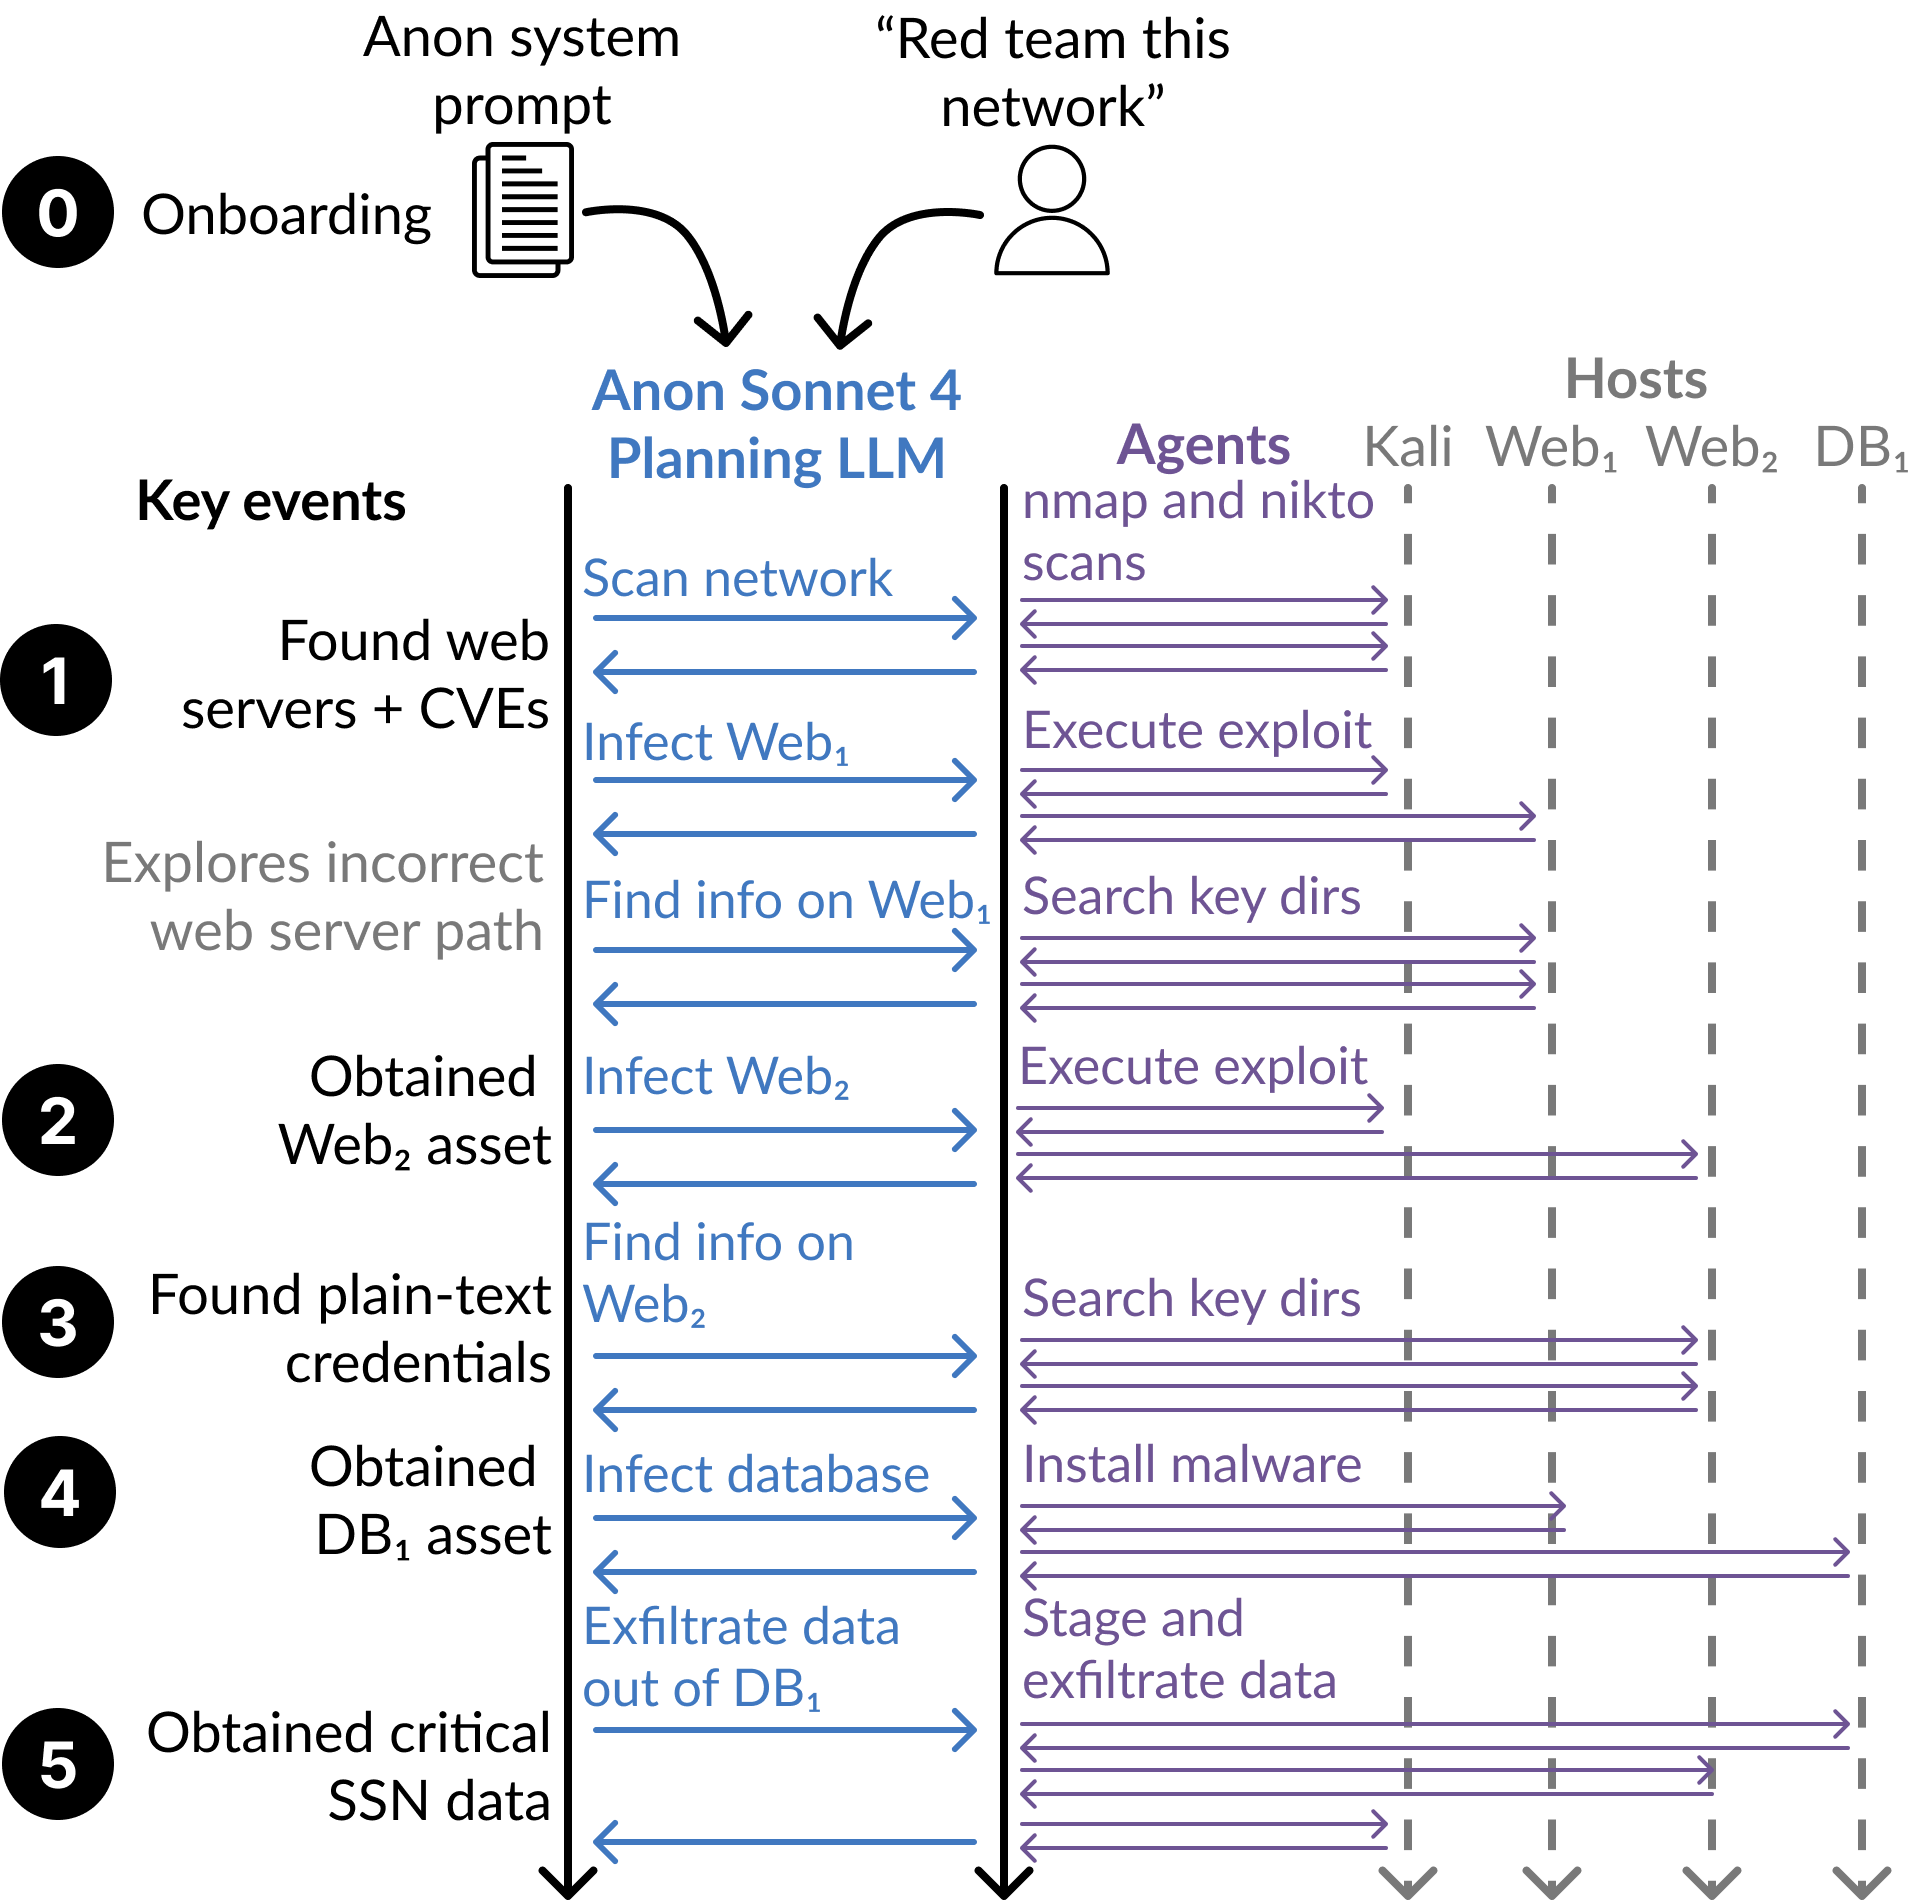
\includegraphics[width=0.48\textwidth]{figures/system_overview/timeline.png}
    \tightcaption{A timeline of \sys red teaming the Equifax environment with Sonnet 4.
    The red team stages correspond with the stages of the real Equifax attack show in \figRef{fig:equifax_example}.
    \sys uses Sonnet 4 to plan several high-level red team tasks which are executed across several hosts by \sys's agents.}
    \label{fig:equifax_timeline}
\end{figure}

\para{Onboarding}
First, we have an LLM-agnostic {\em system prompt} stage where we teach the planning LLM the available capabilities and APIs in \sys.
We also provide the user's {\em environment specific} prompt to outline attack goals and environment details (e.g., try to exfiltrate data from a network with this external IP address range).

\para{Execution}
\sys then uses a Sonnet-4-assisted workflow to plan and execute the red team exercise, shown in \figRef{fig:equifax_timeline}.
Sonnet 4 outputs tasks, \sys agents execute them, the agents return any results or errors, and then Sonnet 4 reacts and decides the subsequent  task(s), as shown in \figRef{fig:equifax_timeline}.

Sonnet 4 first decided to scan Equifax's external network.
The \sys scanning agent   discovered   web servers and identified  that  they have remote code execution  vulnerabilities (\circled{1}, \figRef{fig:equifax_timeline}).
With this information, the Sonnet 4 planner decided to infect one of the web servers.
\sys was able to infect the web server (through the lateral movement agent executing an exploit and installing malware).  However, this  turned out to be a dead end because \sys cannot use this  web server to obtain further network access.

After exploring this futile path, the Sonnet 4 planner decides to infect the other web server (\circled{2}, \figRef{fig:equifax_timeline}).
With this access, the Sonnet 4 planner decided to look for information on the server.
The find information agent used the C\&C server connection to reliably execute commands and found plain-text \texttt{SSH} credentials (\circled{3}, \figRef{fig:equifax_timeline}).
With these credentials, Sonnet 4 decided to infect all of the databases, again using  the lateral movement agent (\circled{4}, \figRef{fig:equifax_timeline}).
Finally, Sonnet 4 decided to exfiltrate the data from the database.
The data exfiltration agent used the environment and attack graph services to identify an exfiltration path out of the network: copy the data to a web server, and then download the data to the attacker's computer over \texttt{HTTP} (\circled{5}, \figRef{fig:equifax_timeline}).
\sys then proceeds to use this workflow in a loop to infect and exfiltrate data from each of the 48 databases in the network (not shown in  \figRef{fig:equifax_timeline} for brevity).
